\documentclass[tikz,border=3.14mm]{standalone}
\usepackage[utf8]{inputenc}
\usepackage[english]{babel}
\usepackage{amsfonts,verbatim,graphicx,url}
\usepackage{cite}
\usepackage{mathtools}
\usepackage{amsmath}

\usepackage{standalone}
\usepackage{graphicx}
\usepackage{caption}
\usepackage{nomencl}
\usepackage{listings}
\usepackage{rotating}
\usepackage{tikz}
\usetikzlibrary{shapes,arrows}
\usepackage{subfig}


\tikzstyle{MRI} = [ultra thick, fill=blue, ellipse, minimum width=10pt,
    align=center, text=white, text width=0.8cm,text centered ]
    \tikzstyle{MRIX} = [ultra thick, fill=purple, ellipse, minimum width=10pt,
    align=center, text=white,text width=0.8cm,text centered]
\tikzstyle{block} = [rectangle, draw,  
 text width=5em,  rounded corners, minimum height=4em]
\tikzstyle{lineX} = [draw,line width=2mm, blue, -latex']
\tikzstyle{lineMRI} = [draw,line width=2mm, blue]
\tikzstyle{lineR} = [draw,line width=3mm, red, -latex']
\tikzstyle{lineMRIR} = [draw,line width=2mm, red]
\tikzstyle{init} = [rectangle, draw, fill=blue!20, 
 text width=0.9*\textwidth, text centered, rounded corners, minimum height=4em]

\tikzstyle{writing} = [rectangle, draw,opacity=0,text opacity=1, anchor=west,text width=0.9*\textwidth ]
\tikzstyle{underscore} = [draw,line width=1mm, blue]
\usetikzlibrary{decorations.pathreplacing,positioning, arrows.meta,calc}

\begin{document}

%\begin{titlepage} \begin{center} \vspace*{1cm} \Huge \textbf{Accumulated Plastic Strain Program} \vspace{0.5cm} \LARGE \vspace{1.5cm} \\ by \\ Lars Magnus Valnes \\\vspace{6.5cm} \includegraphics[width=5cm]{NTNU.png} \vfill Master Thesis\\ \vspace{0.4cm} \Large Department of Physics \\ Norwegian University of Science and Technology\\ June 23, 2014\\ \end{center} \end{titlepage}


\noindent
\begin{tikzpicture}
 
%%%%%%%%%%%%%%% FISRT BOX
\node [block,draw=blue!50, line width=3mm, minimum width =6cm,minimum height =3cm] (MRI data) at (0,1) {};
\node [block,draw=blue!50,fill=white!10 ,line width=1.5mm, minimum width =3cm,minimum height =0.6cm] (MRI data header) at (0,2.5) {MRI Data};
\node[ rectangle,align=center, minimum width =2.5cm ,  draw,opacity=0,text opacity=1 ] (boxtxt1) at (0.0, 1.3) 
{Chapter 3 \& 5 \\ Extracting \\ T1, T2 and DTI. };




%%%%%%%%%%%%%%%%%%%%%%%%%%%%%%%%%%%%%%%%%%%%

%%%%%%%%%%%%% SECOND BOX
\node [block,draw=blue!50, line width=3mm, minimum width =9cm,minimum height =3.5cm] (Freesurfer double) at (0,-3.0) {};

\node [block,draw=blue!50,fill=white!10 ,line width=1.5mm, minimum width =3.5cm,minimum height =0.55cm] (Freesurfer header) at (0,-1.3) {\hspace{0.9mm}FreeSurfer};


%%%%%%%%%%%%%%%%%%%%%%%%%%%%%%%%%%%%%%%%

\node [block,draw=blue!50, line width=1mm, minimum width =3.5cm,minimum height =2.5cm] (DTI) at (-2.1,-3.25) {};

\node [block,draw=blue!50,fill=white!10 ,line width=1.mm, minimum width =1.5cm,minimum height =0.55cm] (DIT header) at (-2.1,-2.0) {\hspace{5mm}DTI};



\node[ rectangle,align=right, minimum width =2.5cm , text width=2.4cm,  align=right,  draw,opacity=0,text opacity=1 ] (boxtxt1) at (-2.0, -2.9) 
{Chapter 5 \\ mri\_convert \\ dt\_recon };

%%%%%%%%%%%%%%%%%%%%%%%%%%%%%%%%%%%%%%%%5
\node [block,draw=blue!50, line width=1mm, minimum width =3.5cm,minimum height =2.5cm] (Seg) at (2.1,-3.25) {};

\node [block,draw=blue!50,fill=white!10,text width=2.4cm, align=center ,line width=1.mm, minimum width =2.5cm,minimum height =0.55cm] (Freesurfer header) at (2.1,-2.0) {Segmentation};

\node[ rectangle,align=left, minimum width =2.5cm ,  text width=3.8cm, align=left,draw,opacity=0,text opacity=1 ] (boxtxt1) at (2.4, -2.9) 
{ Chapter 3 \& 4\\ recon\_all \\ mri\_binarize };

%%%%%%%%%%%%%%%%%%%%%%%%%%%%%%%%%%%%%%%%%%%
\node [block,draw=blue!50, line width=3mm, minimum width =4.2cm,minimum height =3.8cm] (SVMTK) at (2.4,-7.5) {};

\node [block,draw=blue!50,fill=white!10 ,line width=1.5mm, minimum width =1.5cm,minimum height =0.55cm] (SVMTK header) at (2.3,-5.6) { \hspace{0.1cm} SVMTK};
\node[ rectangle,align=left, minimum width =2.5cm ,text width=3.8cm, align=left ,draw,opacity=0,text opacity=1 ] (boxtxt4) at (2.6, -6.8) 
{ Chapter 4 \\ Surface repair \\ Mesh generation \\ Mesh tags };


\node [block,draw=blue, line width=1mm, minimum width =2.8cm,minimum height =1.0cm] (MEshio) at (2.0,-8.6) {};

\node [block,draw=blue,fill=white!10 ,line width=1.mm, minimum width =1.5cm,minimum height =0.4cm,text width=1cm, align=left] (meshio header) at (2.0,-8.1) {meshio};

\node[ rectangle,align=left, minimum width =2.6cm ,text width=3.8cm, align=left ,draw,opacity=0,text opacity=1 ] (boxtxt4) at (2.6, -8.6) 
{Mesh conversion  };

\node [block,draw=blue!50, line width=3mm, minimum width =4.2cm,minimum height =3.8cm] (temp) at (-2.4,-7.5) {};

\node [block,draw=blue!50,fill=white!10 ,line width=1.5mm,text width=3.5cm, align=center, minimum width =3.5cm,minimum height =0.55cm] (temp header) at (-2.4,-5.6) {Nibabel \& Numpy};


\node[ rectangle,align=right, minimum width =2.5cm ,text width=3.3cm, align=right, draw,opacity=0,text opacity=1 ] (boxtxt5) at (-2.5, -6.6) 
{ Chapter 5 \\
  prep\_tensor.py \\
  dti2dolfin.py 



};


%\node[ rectangle,align=right, minimum width =2.5cm ,  draw,opacity=0,text opacity=1 ] (boxtxt5) at (-1.5, -7.8) {dolfin mesh \\ w/ meshio};

\node [block,draw=blue!50, line width=3mm, minimum width =6cm,minimum height =3cm] (FEnics) at (0,-11.5) {};

\node [block,draw=blue!50,fill=white!10 ,line width=1.5mm, minimum width =2.5cm,minimum height =0.55cm] (Fenics header) at (0,-10) {\hspace{3mm}FEniCS};

\node[ rectangle,align=left, minimum width =2.5cm ,  draw,opacity=0,text opacity=1 ] (boxtxt5) at (-1.0, -11.4) 
{Chapter 4 \& 6\\ Scalar diffusion PDE \\ Tensor diffusion PDE\\   };




\draw[lineX] ($(-2.3,-0.)$) -- ($(-2.3,-1.8)$);
\draw[underscore]($(-0.5,-0)$)--($(-2.5,-0)$);
\node[ rectangle, draw,opacity=0,text opacity=1 ] (Txt1) at (-1.55, 0.2) 
{DTI images};

\draw[lineX] ($(2.3,-0.)$) -- ($(2.3,-1.8)$);
\draw[underscore]($(0.0,0)$)--($(2.6,0)$);
\node[ rectangle, draw,opacity=0,text opacity=1 ] (Txt2) at (1.3, 0.2) 
{T1 \& T2 images};


\draw[lineX] ($(0.7,-3.7)$) -- ($(-0.7,-3.7)$);
%\draw[underscore] ($(0.7,-3.9)$) -- ($(0.7,-4.15)$);
%\draw[underscore]($(0.7,-3.75)$)--($(2.2,-3.75)$);
%\node[ rectangle, draw,opacity=0,text opacity=1 ] (TextD1) at (1.5, -3.6) {output};

\draw[lineX] ($(2,-4.3)$) -- ($(2,-5.4)$);
\draw[underscore]($(0.7,-4.3)$)--($(2.2,-4.3)$);
\node[ rectangle, draw,opacity=0,text opacity=1 ] (TextD1) at (1.5, -4.1) 
{surfaces};

\draw[lineX] ($(-2,-4.3)$) -- ($(-2,-5.4)$);
\draw[underscore]($(-0.7,-4.3)$)--($(-2.6,-4.3)$);
\node[ rectangle, draw,opacity=0,text opacity=1 ] (TextD1) at (-1.7, -4.1) 
{tensor.nii.gz};



\draw[lineX]      ($(0.6,-8.3)$) -- ($(-0.6,-8.3)$);
%\draw[underscore] ($(0.7,-8.4)$) -- ($(0.7,-8.75)$);
%\draw[underscore] ($(0.7,-8.0)$)--($(1.7,-8.0)$);
%\node[ rectangle, draw,opacity=0,text opacity=1 ] (TextD1) at (1.2, -7.8) {mesh};




\draw[lineX] ($(2,-9.1)$) -- ($(2,-10.0)$);

%\draw[underscore]($(0.7,-8.7)$)--($(2.2,-8.7)$);
%\node[ rectangle, draw,opacity=0,text opacity=1 ] (TextD1) at (1.5, -8.5) {mesh};

\draw[lineX] ($(-2,-9.)$) -- ($(-2,-10.0)$);


\draw[underscore]($(-0.6,-9.0)$)--($(-3.0,-9.0)$);
\node[ rectangle, draw,opacity=0,text opacity=1 ] (TextD1) at (-1.8, -8.8) 
{mesh w/ tensor};



\node[circle,draw,fill=white!10 ,minimum width=2.25cm ,draw=blue!50,line width=1.0mm,
      path picture={   \node at (path picture bounding box.center){ 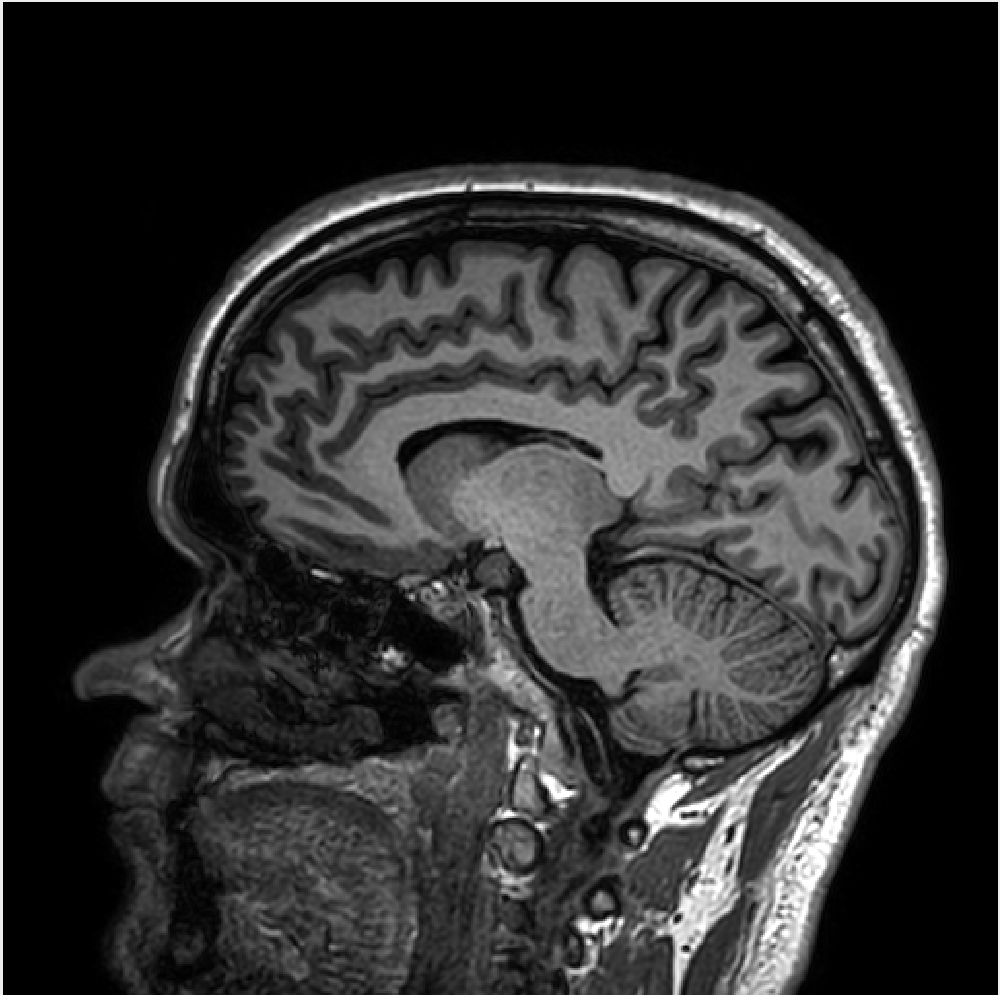
\includegraphics[scale=0.07]{T1-saggital-image.png}}; } ] (T1) at (3.0,1.5){
                   
               };
\node[circle,draw,fill=white!10 ,minimum width=2.25cm ,draw=blue!50,line width=1.0mm,
      path picture={  \node at (path picture bounding box.center){ 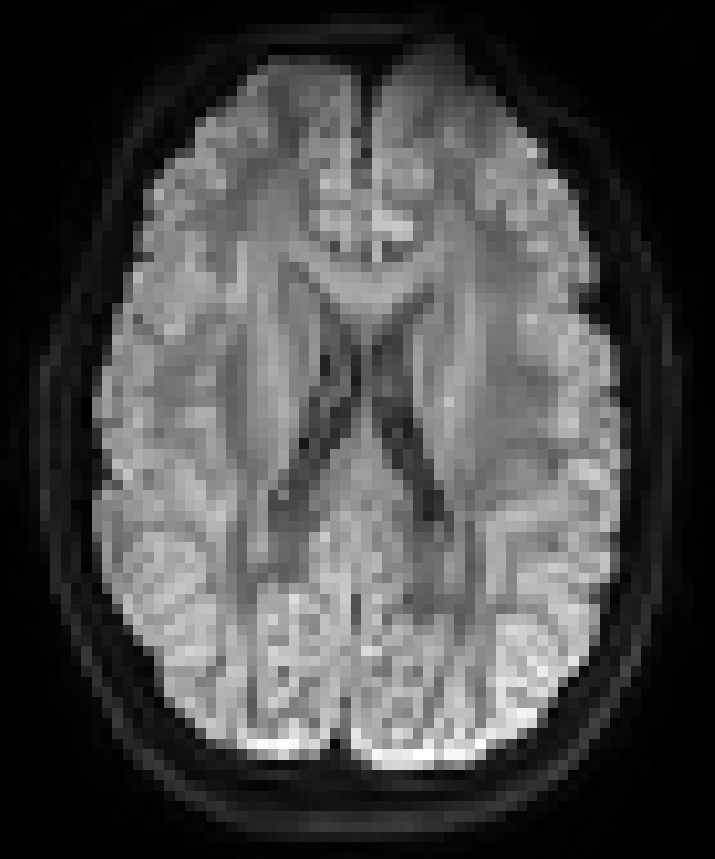
\includegraphics[scale=0.095]{DTI-slice-image-crop}}; } ] (DT1-1) at (-3.0,1.5){
                   
               };
               
\node[circle,draw,fill=white!10 ,minimum width=2.5cm ,draw=blue!50,line width=1.0mm,
      path picture={   \node at (path picture bounding box.center){ 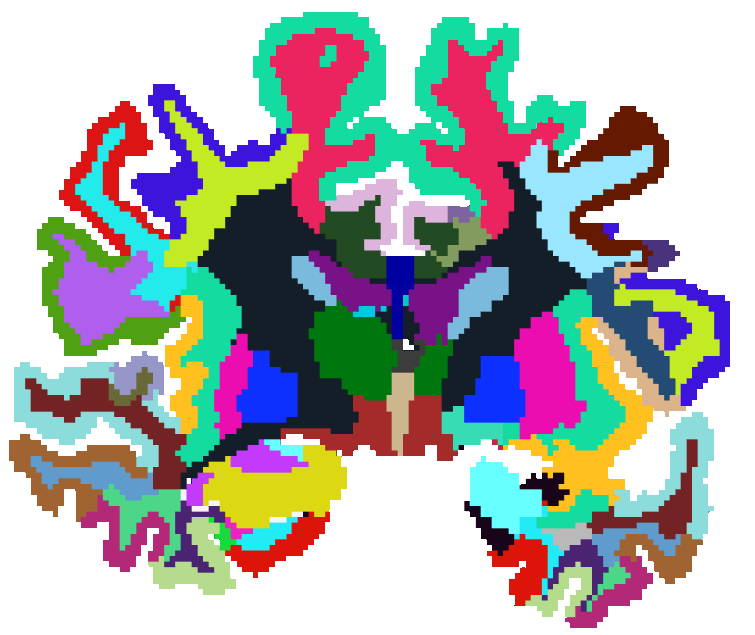
\includegraphics[scale=0.1]{../../chp4/FIG/parcellation-coronalwhiteBG_2.png}}; } ] (parc) at (4.0,-3.65){
                   
               };
\node[circle,draw,fill=white!10 ,minimum width=2.7cm ,draw=blue!50,line width=1.0mm,
      path picture={   \node at (path picture bounding box.center){ 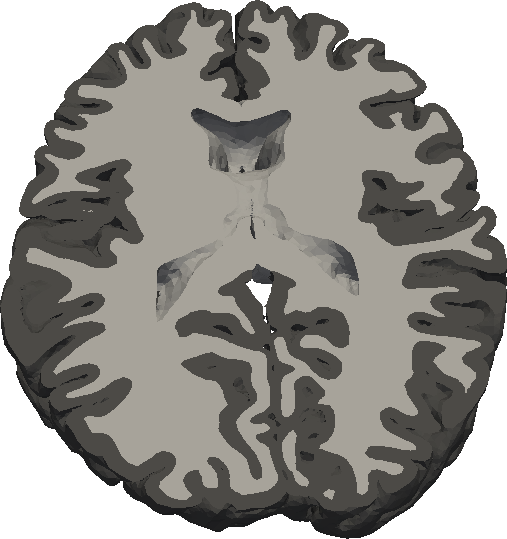
\includegraphics[scale=0.12]{../../chp4/FIG/ernie-fullbrain-crop-b.png}}; } ] (MESH) at (4.7,-7.5){                   
               };


\node[circle,draw,fill=white!10 ,minimum width=2.6cm ,draw=blue!50,line width=1.0mm,
      path picture={   \node at (path picture bounding box.center){ 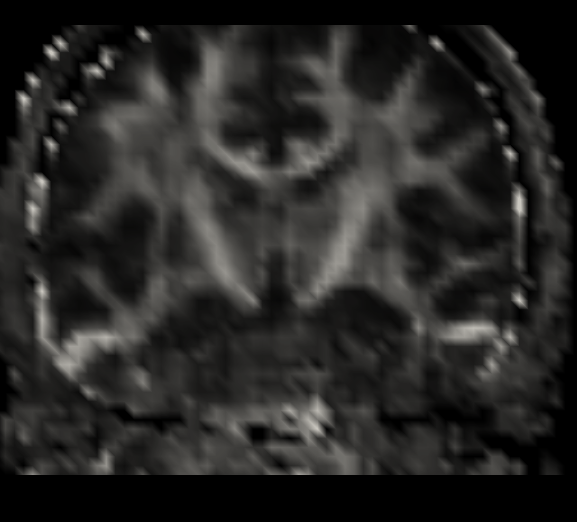
\includegraphics[scale=0.14]{../../chp5/FIG/fa.png}}; } ] (MESH) at (-4.0,-3.65){
                   
               };

\node[circle,draw,fill=white!10 ,minimum width=3.0cm ,draw=blue!50,line width=1.0mm,
      path picture={   \node at (path picture bounding box.center){ 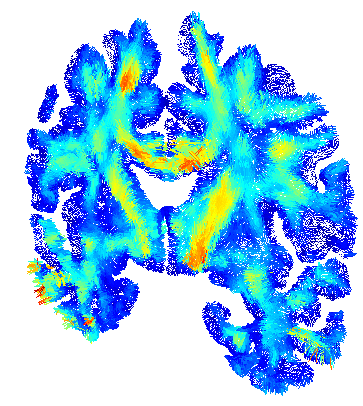
\includegraphics[scale=0.17]{../../chp5/FIG/fiber-dti.png}}; } ] (MESH) at (-4.5,-7.5){
                   
               };


\node[circle,draw,fill=white!10 ,minimum width=3.0cm ,draw=blue!50,line width=1.0mm,
      path picture={   \node at (path picture bounding box.center){ 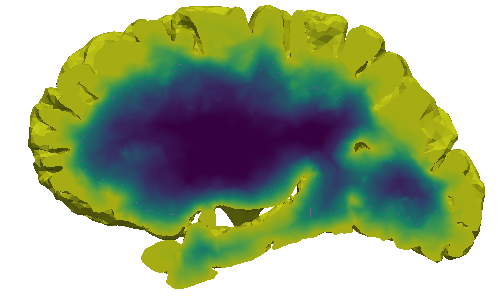
\includegraphics[scale=0.15]{../../chp3/FIG/mri-tracer/48h.png}}; } ] (MESH) at (3.0,-12){
                   
               };


\end{tikzpicture}




\end{document}
